%%%%%%%%%%%%%%%%%%%%%%%%%%%%%%%%%%%%%%%%%
% a0poster Portrait Poster
% LaTeX Template
% Version 1.0 (22/06/13)
%
% The a0poster class was created by:
% Gerlinde Kettl and Matthias Weiser (tex@kettl.de)
% 
% This template has been downloaded from:
% http://www.LaTeXTemplates.com
%
% License:
% CC BY-NC-SA 3.0 (http://creativecommons.org/licenses/by-nc-sa/3.0/)
%
%%%%%%%%%%%%%%%%%%%%%%%%%%%%%%%%%%%%%%%%%

%----------------------------------------------------------------------------------------
%	PACKAGES AND OTHER DOCUMENT CONFIGURATIONS
%----------------------------------------------------------------------------------------

\documentclass[a0,portrait]{a0poster}
\usepackage[font=small,labelfont=bf]{caption}
\usepackage{multicol} % This is so we can have multiple columns of text side-by-side
\columnsep=50pt % This is the amount of white space between the columns in the poster
\columnseprule=0pt % This is the thickness of the black line between the columns in the poster
\usepackage{easySymbols}
\usepackage{wrapfig}
\usepackage[svgnames]{xcolor} % Specify colors by their 'svgnames', for a full list of all colors available see here: http://www.latextemplates.com/svgnames-colors
\usepackage[utf8]{inputenc}
\usepackage{times} % Use the times font
%\usepackage{palatino} % Uncomment to use the Palatino font

\usepackage{graphicx} % Required for including images
\graphicspath{{figures/}} % Location of the graphics files
\usepackage{booktabs} % Top and bottom rules for table
\usepackage[font=small,labelfont=bf]{caption} % Required for specifying captions to tables and figures
\usepackage{amsfonts, amsmath, amsthm, amssymb} % For math fonts, symbols and environments
\usepackage{wrapfig} % Allows wrapping text around tables and figures

\begin{document}

%----------------------------------------------------------------------------------------
%	POSTER HEADER 
%----------------------------------------------------------------------------------------

% The header is divided into two boxes:
% The first is 75% wide and houses the title, subtitle, names, university/organization and contact information
% The second is 25% wide and houses a logo for your university/organization or a photo of you
% The widths of these boxes can be easily edited to accommodate your content as you see fit

\begin{minipage}[b]{0.75\linewidth}
\veryHuge \color{NavyBlue} \textbf{Large Scale Gene Regulatory Network Inference} \color{Black}\\ % Title
\Huge\textit{to uncover Oncogenic Mechanisms}\\[2cm] % Subtitle
% \huge \textbf{John Smith \& James Smith}\\[0.5cm] % Author(s)
% \huge University and Department Name\\[0.4cm] % University/organization
% \Large \texttt{john@LaTeXTemplates.com} --- 1 (000) 111 1111\\
\huge \textbf{ Daniel Morgan$^1$, Deniz Seçilmiş$^1$, Andreas Tj\"{a}rnberg$^2$, Torbj\"{o}rn  Nordling$^3$, Sven Nelander$^4$, Erik Sonnhammer$^1$ } \\[0.1cm]
\large $^1$\it {DBB, Stockholm University \& SciLifeLab} $^2$\it{Department of Bioinformatics, Link\"{o}ping University} $^3$\it {Mechanical Engineering, National Cheng Kung University} $^4$\it {Immunology, genetic and pathology, IGP, Science for Life Laboratory, Uppsala, Sweden
}\\[0.4cm]
\Large \texttt{Daniel.Morgan@SciLifeLab.se, Deniz.Secilmis@SciLifeLab.se}
\end{minipage}
%
% \begin{minipage}[b]{0.25\linewidth}
% 
\includegraphics[width=10cm]{logo.png}\\
% \end{minipage}

\vspace{1cm} % A bit of extra whitespace between the header and poster content

%----------------------------------------------------------------------------------------

\begin{multicols}{2} % This is how many columns your poster will be broken into, a portrait poster is generally split into 2 columns

%----------------------------------------------------------------------------------------
%	ABSTRACT
%----------------------------------------------------------------------------------------

\color{Navy} % Navy color for the abstract

\section*{abstract}

Inferring a gene regulatory network (GRN) from knockdown experiments can give insight into specific mechanisms directing cellular behavior. In order to explore the differences among human cancer GRNs, we infer networks from 9 human cancer and 2 stem cell cell-lines using public single gene knockdown data characterized by the highly multiplexed L1000 platform and cleared of unwanted variation via FC1000. The NestBoot inference protocol is implemented to infer reliable a GRN per cell line by restricting the inclusion of false links. A composite of all individual gene knockdown data is used to find a network of regulatory elements common among all the cell lines. Finally, a jaccardian all-versus-all comparison is made to contrast specific regulators within each cell line to those omnipresent in the composite network. The results confirm many relational elements per specific oncogenic subtype, as well as novel regulations predicted across and within each cell line.



%----------------------------------------------------------------------------------------
%	INTRODUCTION
%----------------------------------------------------------------------------------------

\color{SaddleBrown} % SaddleBrown color for the introduction

\section*{Introduction}

The influential capability among biological components within a system is captured in a gene regulatory networks (GRN), used here to model cellular behavior with the aim of identifying functional subsets of genes. Accurately identifying these interactions is an ongoing challenge. Information can be added to the system enabling more accurate inference in the form of a design matrix by defining perturbations occurring before characterization, a unique feature lacking in mutual information or tree building methods such as CLR\cite{faith2007large} or Genie3\cite{GENIE3}, respectively. However, datasets meeting these many experimental requirements are a somewhat rarity.

A newly developed platform, L1000 \cite{subramanian2017next}, enabled genetic experiments on a larger scale than previously available to the scientific community. Experimental replicates were maintained and normalized, removing unwanted variation using FC1000 \cite{lonnstedt2017fc1000}. For any inferred network to be reliable, each relationship necessitates high accuracy and reliability. For this reason we enlist our regression based inference protocol to model the underlying interactions controlling the intracellular activity of several cancer variants. This generalized framework returns networks of high accuracy and reproducibility by controlling FDR. %The interactions recovered include links essential for sustained life and growth in the cancer models, but also those which dictate the progression of cellular development, potential indicators to their collective role in oncogenic progression.

%----------------------------------------------------------------------------------------
%	OBJECTIVES
%----------------------------------------------------------------------------------------

\color{DarkSlateGray} % DarkSlateGray color for the rest of the content

\section*{Main Objectives}

\begin{enumerate}
\item Removed batch and other sources of unwanted noise from L1000 dataset.
\item Infer networks per cell line \& as a {\it generic} aggregate.
\item Compare subtype networks link-wise.
\item Investigate liver cancer subnetwork.
\end{enumerate}

%----------------------------------------------------------------------------------------
%	MATERIALS AND METHODS
%----------------------------------------------------------------------------------------

\section*{Materials and Methods}
% \headerbox{Materials}{name=materials,column=3,below=introduction}{

\begin{multicols}{2}
% \begin{table}[]
% \begin{center}
% \begin{minipage}[t]{0.5\textwidth}
\begin{tabular}{@{}llllll@{}}
\toprule
\textbf{Cell line} & \textbf{genes} & \textbf{expts} & \textbf{SNR} & \textbf{cond.\#} \\ \midrule
A375 &  904 & 2769 & 0.0015 & 89 \\
A549 &  903 & 2502 & 0.0025 & 47 \\
HA1E &  828 & 2405 & 0.0021 & 44 \\
HCC515 &  872 & 2642 & 0.0019 & 40 \\
HEPG2 &  766 & 2478 & 0.0025 & 38 \\
HT29 &  829 & 3179 & 0.0024 & 30 \\
MCF7 &  830 & 2138 & 0.0014 & 66 \\
PC3 &  837 & 2092 & 0.0017 & 59 \\
VCAP &  905 & 2435 & 0.0013 & 91 \\
ASC & 752 & 2612 & 0.0051 & 19 \\
NPC & 752 & 2737 & 0.0029 & 36 \\
generic & 551 & 10203 & 0.0156 & 22 \\ \bottomrule \\
\end{tabular}
% \end{minipage}
% \end{center}

%------------------------------------------------
% \begin{center}
% \begin{minipage}[t]{0.5\textwidth}
\subsection*{Mathematical Section}

\textbf{Model:} $  \mY = -\mA^{-1}(\mP +\mF) + \mE$\\
\textbf{Y}: expression data\\
\textbf{A}: network\\
\textbf{P}: perturbation matrix\\
\textbf{E}: input noise estimate\\
\textbf{F}: output noise estimate\\

% \begin{center}
% \resizebox{0.9\textwidth}{!}{\begin{minipage}{\textwidth}
\begin{tabular}{l l l l}
\toprule
\textbf{Method} & \textbf{Equation} \\
\midrule
LS & $\{ \hat{A}_{ls},\Delta _{ls} \}: = \arg \min\limits_{X,\Delta A} ||\Delta A||_F$ \\ 
& $\hat{A}_{OLS} = {{(X^TX)}^{-1} X^Ty}$ \\ \\

\end{tabular}
% \end{minipage}
% \end{center}
\end{multicols}

\begin{center} \vspace{.15cm}
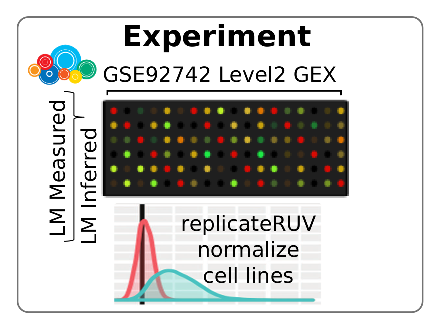
\includegraphics[width=.45\linewidth]{L1000_method_1.eps}
\hspace{.25cm}\vspace{.1cm}

\includegraphics[width=.5\linewidth]{L1000_method_2.eps}
\end{center}
\vspace{-.3cm}

%----------------------------------------------------------------------------------------
%	RESULTS 
%----------------------------------------------------------------------------------------

\section*{Results}
\begin{multicols}{2}
% \begin{center}
% \resizebox{0.9\textwidth}{!}{\begin{minipage}{\textwidth}
\begin{tabular}{@{}lllll@{}}
\toprule
\textbf{Network} & \textbf{tissue} & \textbf{links} & \textbf{sparsity} & \textbf{links/gene} \\ \midrule
A375 & melanoma & 2675 & 0.0033 & 2.96 \\
A549 & lung & 1883 & 0.0023 & 2.09 \\
HA1E & kidney & 2353 & 0.0034 & 2.84 \\
HCC515 & lung & 3577 & 0.0047 & 4.10 \\
HEPG2 & liver & 2880 & 0.0049 & 3.76 \\
HT29 & colon & 2879 & 0.0042 & 3.47 \\
MCF7 & breast & 3185 & 0.0046 & 3.84 \\
PC3 & prostate & 3978 & 0.0057 & 4.75 \\
VCAP & prostate & 2233 & 0.0027 & 2.47 \\
ASC & adipocyte SC & 1054 & 0.0019 & 1.40 \\
NPC & CNS iPSC & 2473 & 0.0044 & 3.29 \\
generic & ---- & 1645 & 0.0054 & 2.99 \\\bottomrule \\
\end{tabular}
% \end{minipage}}
% \end{center}


% \begin{figure}
% \hspace{.25cm}\vspace{.1cm}
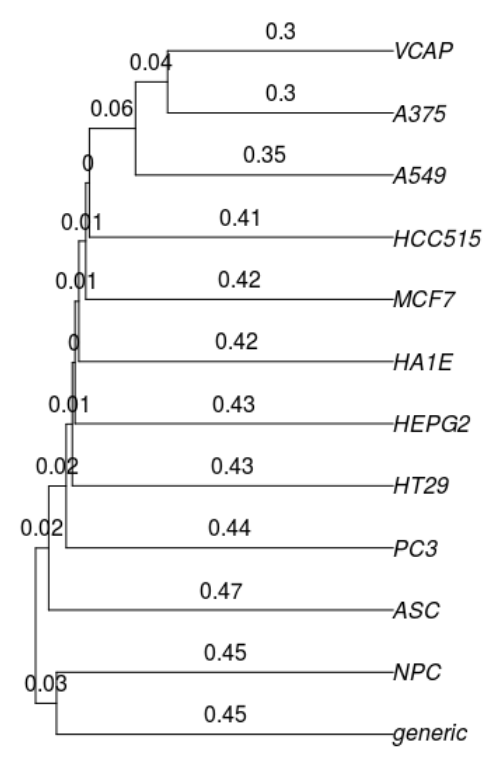
\includegraphics[width=.75\linewidth]{L1000_jiccard.png}
% \end{figure}
\end{multicols}

\begin{center}
\hspace{.25cm}\vspace{.1cm}
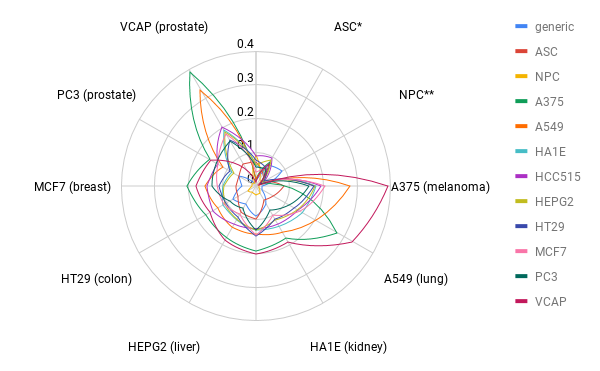
\includegraphics[width=1\linewidth]{L1000_spider.png}
% \caption{{\textbf Comparing network links}using Jaccard distance.}
\end{center}
\vspace{-.3cm}
%----------------------------------------------------------------------------------------
%	CONCLUSIONS
%----------------------------------------------------------------------------------------

\color{SaddleBrown} % SaddleBrown color for the conclusions to make them stand out

\section*{Conclusions}

\begin{itemize}
\item The FC1000 normalized GSE92742 data contains replicate experiments which may be useful to the wider scientific community beyond those interested in network inference as replicates can offer measures of variance. 
\item The RUV FC1000 process removes certain experimental replicates, reducing noise and providing a more uniform PCA.
\item Inferring networks allows investigation of both elements common and unique to cancers, and to SC as well.
\item Tissue-specific subnetworks offer predicted disease mechanisms.
\end{itemize}

\color{DarkSlateGray} % Set the color back to DarkSlateGray for the rest of the content

%----------------------------------------------------------------------------------------
%	FORTHCOMING RESEARCH
%----------------------------------------------------------------------------------------

\section*{Forthcoming Research}

Incorporation of small molecule perturbation may offer novel drug-target predictions for each cancer subtype.

 %----------------------------------------------------------------------------------------
%	REFERENCES
%----------------------------------------------------------------------------------------

% \nocite{*} % Print all references regardless of whether they were cited in the poster or not
\bibliographystyle{plain} % Plain referencing style
\bibliography{references.bib} % Use the example bibliography file sample.bib

%----------------------------------------------------------------------------------------
%	ACKNOWLEDGEMENTS
%----------------------------------------------------------------------------------------

\section*{Acknowledgements}

SSF Systembiologi Grant 2016.

%----------------------------------------------------------------------------------------

\end{multicols}
\end{document}